\chapter{Design Decisions}

\section{Mean Reversion Strategies}
Considering the current state of the art and the limited exploration of statistical arbitrage in decentralised exchanges, the objective of this project is to examine the profitability of mean reversion techniques in pairs trading and determine if they offer a viable investment opportunity. Additionally, by employing various methods to estimate the hedge ratio and effectively manage risk, we can further analyse the overall performance and appeal of the trading strategy to potential traders.
\\[3mm]
In the mean reversion strategies, the hedge ratio refers to the ratio or proportion between the positions of two assets involved in a pairs trading strategy. It determines the optimal allocation of capital between the assets to minimise risk and create a market-neutral position. The hedge ratio represents the number of units of one asset that should be bought for each unit of the other asset to be shorted in order to create a balanced or hedged position. It is derived through statistical techniques such as regression analysis. The methods that are explored in this paper are the use of a Constant Hedge Ratio, Sliding Window Ordinary Least Squares, Lagged Ordinary Least Squares, the unrestricted OLS model returned by the Granger Causality Test and also the Kalman Filter. These methods are selected due to their ability to test whether underlying dynamics affect the relationships between liquidity pools, hence affecting the hedge ratio. To further see the details and implementation of each strategy, refer to Section \ref{sec:strats}.

\section{Buying and Short Selling}
\label{sec:buying-selling}
The process of buying and short selling (often called selling) in traditional markets is relatively straightforward, as brokers and exchanges play a crucial role in executing orders on behalf of individuals. However, when it comes to trading cryptocurrencies, the responsibility falls directly on the trader. Therefore, it becomes essential to clearly define what buying and selling entail in the context of cryptocurrency trading.

\subsection{Buying}
Prices on decentralised exchanges are represented as ratios, for example, 1 USDC = $P$ WETH. With this understanding, let us delve into the process of buying one unit of USDC/WETH on a decentralised exchange:
\begin{itemize}
    \item Opening a Buy position:\begin{itemize}
        \item Starts with $P_{0}$ WETH
        \item Swaps the WETH for USDC, hence ends with 1 USDC
    \end{itemize}
    \item Closing a Buy position:\begin{itemize}
        \item Starts with 1 USDC
        \item Swaps the USDC for WETH, hence ends with $P_1$ WETH
    \end{itemize}
\end{itemize}
\noindent Consequently, if the price of USDC/WETH increases from the moment the buy position is opened to the time it is closed, the trader realises a profit. On the other hand, if the price declines during this period, the trader incurs a loss.

\subsection{Short Selling}
Short selling an asset is a more complex process compared to buying because it involves trading an asset the trader does not initially possess. In traditional markets, this consists of the trader borrowing the desired asset from a broker or another party and selling it. When the trader decides to close the position, they repurchase the same amount of the borrowed asset and return it to the lender, hoping that its value has declined. In traditional settings, brokers and exchanges typically automate the borrowing and returning processes. However, in the context of decentralised exchanges (DEXes), such mechanisms are absent or not readily available.
\\[3mm]
To carry out the short-selling process, the utilisation of a lending protocol to borrow any required assets is employed. By leveraging a lending protocol, short-selling becomes easily accessible. The process of selling is as follows:
\begin{itemize}
    \item Opening a Sell position:\begin{itemize}
        \item Borrow 1 USDC
        \item Swaps the USDC for WETH, hence ends with $P_0$ WETH
    \end{itemize}
    \item Closing a Sell position:\begin{itemize}
        \item Starts with $P_0$ WETH
        \item Swaps the WETH for USDC, hence ends with $\frac{P_0}{P_1}$ USDC
        \item Return the borrowed USDC, leaving $\frac{P_0}{P_1} - 1$ USDC
    \end{itemize}
\end{itemize}
Consequently, if the price of USDC/WETH decreases, i.e. $P_1 < P_0$ from the moment the sell position is opened to the time it is closed, the trader realises a profit. On the other hand, if the price increases during this period, the trader incurs a loss.
\\[3mm]
Note that this is an illustrative example and does not account for any potential fees that the trader might incur.


\section{Protocols of Interest}
\subsection{Uniswap}

Uniswap is a decentralised exchange protocol built on the Ethereum blockchain. It allows users to trade ERC-20 tokens directly from their wallets without the need for intermediaries or traditional order books. Uniswap utilises automated market-making, where liquidity providers contribute funds to liquidity pools, earning fees on trades made in the pool. The protocol employs a mathematical formula called the constant product formula to maintain balanced token ratios in the pool. When users want to trade, Uniswap calculates the conversion based on the pool's token ratios and executes the trade through a smart contract.

\subsubsection{Automated Market Maker (AMM) Model and Liquidity Pools}

The AMM model is a system that replaces traditional order books with liquidity pools to facilitate trading between different tokens. Automated Market Makers do this with the aid of liquidity pools. They are pools of tokens contributed by liquidity providers (LPs) to facilitate trading between tokens within the exchange. One paper describes pools as ``a smart contract that holds at least two cryptoassets and allows trading through depositing a token of one type and thereby withdrawing tokens of the other type''~\cite{schar2021decentralized}. These liquidity pools are maintained by smart contracts on Ethereum and Liquidity Providers (LPs). Liquidity providers are individuals that voluntarily contribute an equal amount of cryptocurrencies to liquidity pools; for example, in a pool for trading ETH and DAI, LPs would contribute an equal value of ETH and DAI tokens. LPs are incentivised to provide liquidity in exchange for a share of the trading fees in the liquidity pool. LPs can later withdraw their shares along with the accumulated fees. On Uniswap V3, the fee varies depending on the set-up of the liquidity pool; currently, the fees can be any of the following: 0.01\%, 0.05\%, 0.3\%, or 1\%.

\subsubsection{Constant Product Formula}

The AMM model relies on a mathematical formula called the constant product formula ($xy = k$) to maintain a balanced ratio between the tokens in the pool and calculate the exchange rate. As trades occur, the product of the token balances remains constant. When one token's proportion in the pool decreases, its value increases, ensuring an automatic price adjustment. When a trade is executed, the price change can be described in this formula $(x + \Delta x)(y + \Delta y) = k$. Hence, after rearranging: $\Delta y = \frac{k}{x + \Delta x} - y$. Under this model, the balance of the tokens in a liquidity pool can never be depleted as the token will get infinitely more expensive as the reserves approach 0.

\begin{figure}[!htb]
    \centering
    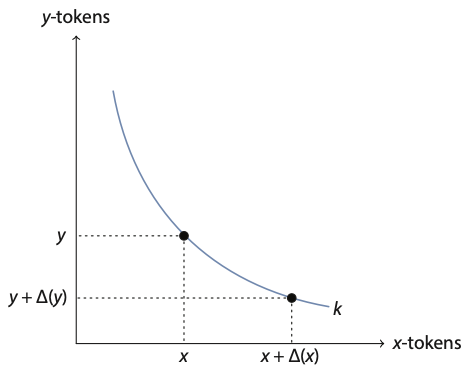
\includegraphics[width=0.5\textwidth]{background/Images/constant_product_formula.png}
    \caption{Constant Product Formula~\cite{schar2021decentralized}}
\end{figure}

\subsubsection{Slippage}

As seen in Figure \ref{fig:uniswap_lp}, we can see how the constant product formula is used in Uniswap. Uniswap allows users to set slippage tolerance levels, determining the maximum acceptable difference between the expected and executed prices. Slippage refers to the difference between the expected price of a trade and the executed price due to market volatility and liquidity conditions. Slippage happens because the constant product formula adjusts prices based on the ratio of tokens in the pool. As trades are executed, token balances and prices change accordingly. Thus, larger trades can cause a more significant price impact, resulting in slippage.

\begin{figure}[!htb]
    \centering
    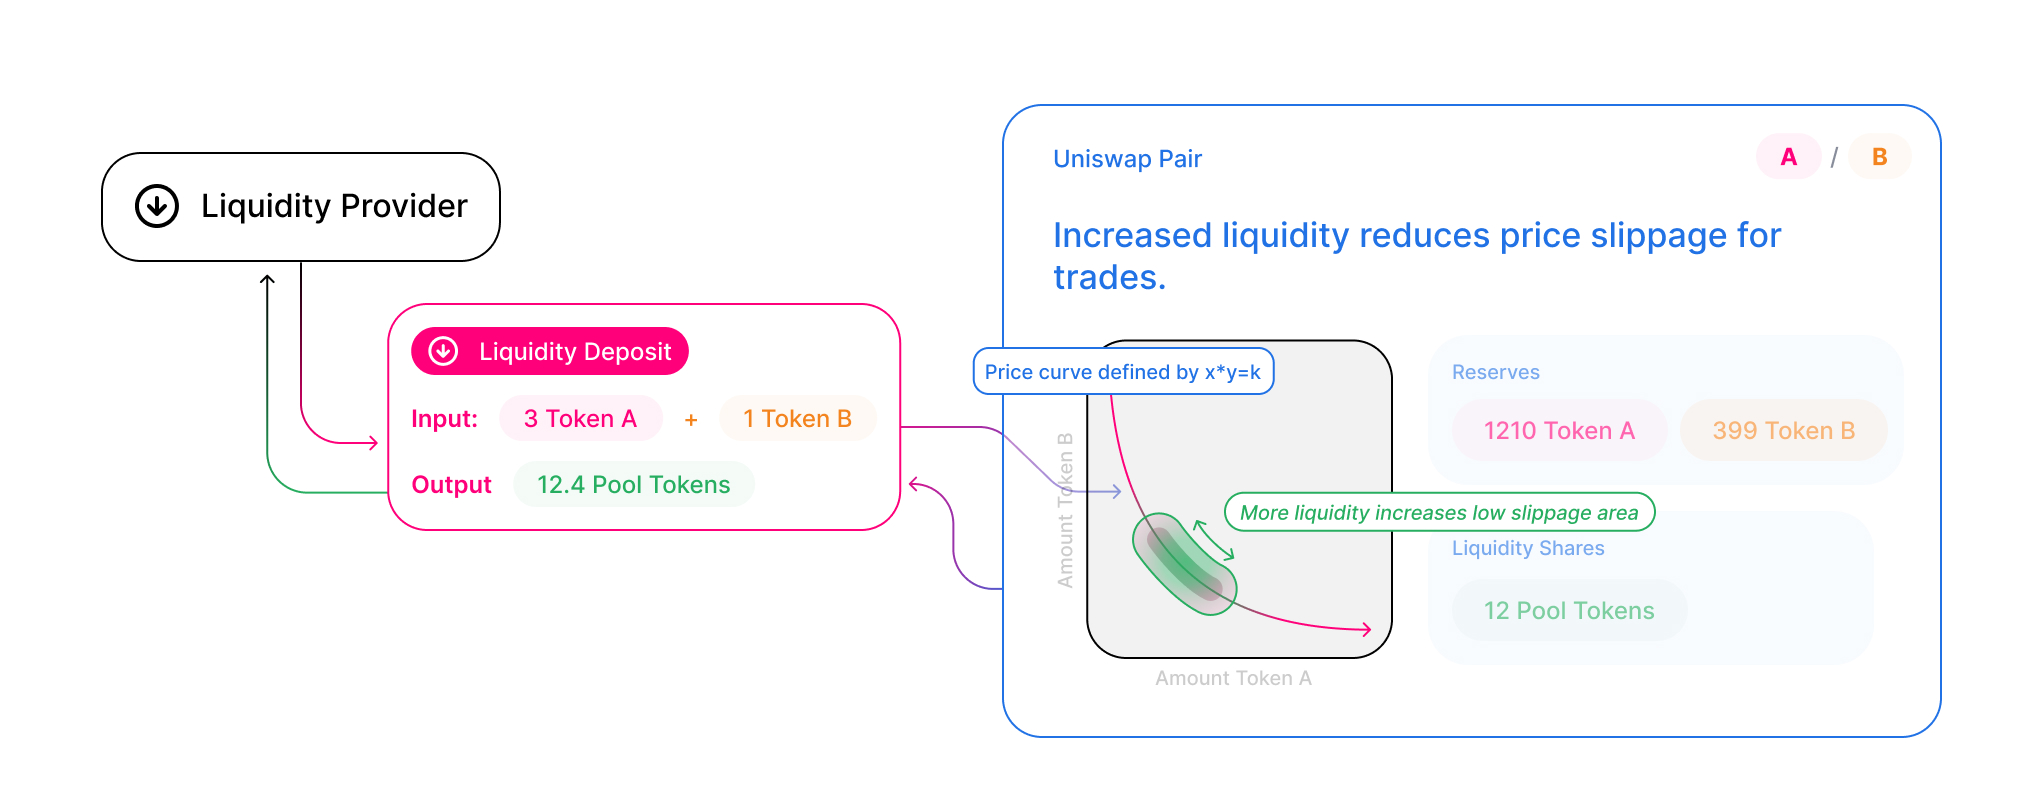
\includegraphics[width=\textwidth]{background/Images/uniswap_lp.jpeg}
    \caption{How Uniswap works~\cite{uniswap} \label{fig:uniswap_lp}}
\end{figure}

\subsection{Aave}

Aave is a decentralised lending and borrowing protocol built on the Ethereum blockchain. It enables users to lend and borrow a wide range of cryptocurrencies directly without the need for intermediaries such as banks. Aave operates through liquidity pools and smart contracts, providing a secure, transparent, and efficient platform for lending and borrowing.
\\[3mm]
Users can deposit their cryptocurrency assets into Aave's liquidity pools and earn interest on their deposits. These funds contribute to the available liquidity for borrowers. On the other hand, borrowers can use their deposited assets as collateral to borrow other assets from the pool. The amount they can borrow is determined by the value of their collateral and specific borrowing parameters set by the protocol.
\subsubsection{Liquidity Pools}
The fundamental mechanism enabling Aave's lending and borrowing functionality is liquidity pools. Users deposit their cryptocurrency assets into Aave's liquidity pools. These assets serve as collateral and contribute to the overall liquidity of the protocol. The deposited assets in the liquidity pools create reserves of available liquidity. These reserves are utilised to fulfil borrowing demands from other users within the Aave ecosystem.
\subsubsection{Lending and Borrowing}
Lending works by lenders depositing their cryptocurrency assets into Aave's liquidity pools. These assets act as collateral and are represented by interest-bearing tokens called aTokens. The aTokens represent the user's share of the deposited assets. Interest is earnt immediately and is accrued in real-time.
\\[3mm]
The borrowing process is enabled by borrowers using their deposited assets as collateral to borrow other assets from the liquidity pools. The value of the collateral determines the borrowing capacity. The borrowing capacity is calculated by parameters set by Aave, one of which is the maximum loan-to-value (LTV) ratio. Once the borrower requests a loan, if the borrower's collateral meets the necessary requirements, they can proceed with the loan and transfer the borrowed funds to the borrower's wallet. In addition, borrowers pay interest on the borrowed amount based on the prevailing interest rates. Aave offers both variable and stable interest rates for borrowers. Variable rates fluctuate based on market dynamics, while stable rates remain fixed. This flexibility allows users to choose the borrowing option that best suits their needs. The interest on a loan is accrued in real-time, second by second, and the borrower decides when to repay it, as long as the loan is safe from liquidation. Liquidation happens if the value of a borrower's collateral falls below the liquidation threshold due to market volatility; the collateral can be liquidated. Liquidators can purchase the collateral at a discounted price to ensure the solvency of the liquidity pool.

\section{Fees that are incurred when trading}
As previously mentioned, when engaging in trading activities, there are several fees that are deducted. These fees serve multiple purposes, including compensating the liquidity providers and addressing the potential lack of access to assets from the lender. Therefore, in this section, we will delve into the various costs associated with implementing and executing the strategy.

\subsection{Gas Fees}
Gas fees in Ethereum are a crucial component of the network's operation. They serve two primary purposes: to prevent spam and denial-of-service attacks and to incentivise miners to include transactions in the blockchain. Each operation, such as sending tokens, executing a smart contract function, or interacting with decentralised applications, consumes a certain amount of gas.
\\[3mm]
The fee is calculated by multiplying the gas price (expressed in Gwei, where 1 Gwei is equal to 0.000000001 ETH) by the gas used~\cite{noauthor_gas_nodate}. As mentioned in previous sections, when a user initiates a transaction, the user specifies the gas limit, which defines the maximum amount of gas that a user is willing to pay for a transaction; if the gas limit is too low and the gas used is more significant than its limit, the transaction will fail and be reverted. This means that the state changes made by the transaction will not be recorded on Ethereum, and the gas fees paid for that transaction will be lost.

\begin{figure}[!htb]
    \centering
    \makebox[\textwidth]{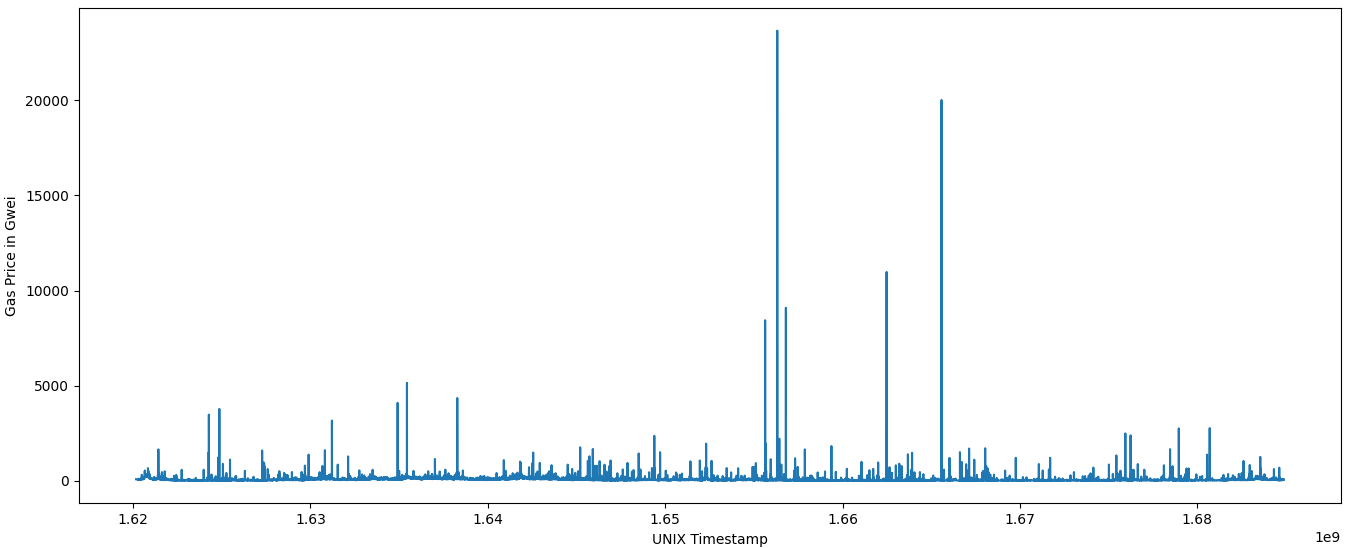
\includegraphics[width=1\textwidth]{project/Images/gas_price_1.png}}
    \caption{The gas price over time}
    \label{fig:gwei_over_time}
\end{figure}

\noindent Figure \ref{fig:gwei_over_time} displays the gas price history over time, showing the price surges and drops. The market forces of supply and demand determine the reason for these fluctuations. It is the amount of Ether a user is willing to pay for each unit of gas consumed in a transaction. Miners can prioritise transactions with higher gas prices and thus are incentivised to include transactions with higher gas prices because they receive the gas fees as a reward for their mining efforts. Therefore, setting a higher gas price increases the chances of a transaction being executed.
\\[3mm]
The second part of the gas fee is how much gas is used; it is calculated by adding the gas used for each operation in the transaction. Each operation has a predefined gas cost associated with it, which reflects the complexity and resource requirements of that operation. When a transaction or smart contract execution is initiated, the Ethereum Virtual Machine (EVM) processes each operation and deducts the corresponding gas cost from the gas limit. In addition to this, Ethereum also has a base fee with all of their transactions; thus, having multiple small transactions becomes more costly than using a large combined transaction~\cite{noauthor_gas_nodate}.

\subsection{Uniswap Fees}
In addition to transaction fees, there is another fee mechanism in place within the system when swapping on Uniswap. This fee is designed to incentivise and reward liquidity providers on the platform. When a swap occurs, a fee is deducted from the tokens expected to be returned to the user.
\\[3mm]
The fee is calculated as a percentage of the swap volume, meaning that the larger the swap, the higher the fee. For example, let us consider a scenario where the exchange price is 1 TKNA = 100 TKNB, and the fee is set at 0.3\%. If someone exchanges 1 TKNA for TKNB, instead of receiving the full 100 TKNB based on the exchange rate, they will receive 100$\times$(1 - 0.3\%) TKNB = 99.7 TKNB. The fee reduces the total amount of tokens received in the swap.
\\[3mm]
It is important to note that the specific fee percentage may vary between different liquidity pools on Uniswap. Each liquidity pool can have its own fee tier, and the fees associated with each interested liquidity pool can be seen in Table \ref{tab:uniswap-fees}.

\begin{table}[!htb]
    \begin{tabular}{|l|l|l|r|}
        \hline
                                      Pool Address & Token0 & Token1 &  Fee Tier as a \% \\\hline\hline
        0x88e6a0c2ddd26feeb64f039a2c41296fcb3f5640 &   USDC &   WETH &     0.05 \\\hline
        0x8ad599c3a0ff1de082011efddc58f1908eb6e6d8 &   USDC &   WETH &     0.30 \\\hline
        0x11b815efb8f581194ae79006d24e0d814b7697f6 &   WETH &   USDT &     0.05 \\\hline
        0x4e68ccd3e89f51c3074ca5072bbac773960dfa36 &   WETH &   USDT &     0.30 \\\hline
        0x60594a405d53811d3bc4766596efd80fd545a270 &    DAI &   WETH &     0.05 \\\hline
        0xc2e9f25be6257c210d7adf0d4cd6e3e881ba25f8 &    DAI &   WETH &     0.30 \\\hline
        0xe0554a476a092703abdb3ef35c80e0d76d32939f &   USDC &   WETH &     0.01 \\\hline
        0xc5af84701f98fa483ece78af83f11b6c38aca71d &   WETH &   USDT &     0.1  \\\hline
    \end{tabular}
    \caption{Uniswap fees for each liquidity pool of interest \label{tab:uniswap-fees}}
\end{table}

\subsection{Aave Fees \& Collatoral}
Aave facilitates lending and borrowing transactions among users, and as part of its operations and incentive mechanisms, it imposes certain fees. In the context of this trading strategy, the only fees applicable would be the interest rates on the loan. The interest rate is typically expressed as an Annual Percentage Yield (APY) and is accrued continuously. Currently, Aave supports variable interest rates, which fluctuate based on market conditions, the borrowed asset, and supply and demand dynamics within Aave.
\\[3mm]
Another aspect of Aave for the trading strategy is collateralisation and the avoidance of liquidation. Liquidation occurs when a borrower's position is forcibly closed, and their collateral assets are sold off in cases of default or insufficient collateral. When borrowing from Aave, borrowers are required to allocate a certain percentage of the loan value as collateral, known as the Loan-to-Value (LTV) ratio~\cite{aave_risk}. For instance, if a token has a 75\% LTV, borrowers can borrow 0.75 ETH worth of the corresponding token for every 1 ETH worth of collateral provided. However, as token prices fluctuate, the ratio between the borrowed token value and the collateral value changes, posing risks for both lenders and Aave. To safeguard lenders and maintain protocol solvency, a liquidation threshold is established. If the collateral value falls below this threshold, the borrower's position becomes vulnerable to liquidation. In such cases, the collateral is auctioned off to repay the outstanding debt to the lenders. Typically, the liquidation threshold is set 5-10\% higher than the asset's LTV. For WETH, the Loan-to-Value ratio is 82.5\%, and the liquidation threshold is 86\%.

\section{Liquidity Pool Pairs of Interest}
\label{sec:liquidity-pools}
One of the remarkable features of Uniswap is its support for even the smallest cryptocurrencies, currently possessing 12,182 liquidity pools.
\\[3mm]
Upon inspection, it can be seen that some pools exhibit high trading volumes, indicating significant activity and demand for those specific pairs. On the other hand, there are also pools with zero liquidity, which could be attributed to various reasons. It could be due to a lack of demand for one of the tokens offered in the pool, or it may indicate that the pool is relatively new and has yet to attract significant participation. Table \ref{tab:liquidity_pools} in the Appendix showcases the diversity of these pools.
\\[3mm]
The mean reversion strategies are centred on certain assertions of the liquidity pools that are being traded on in order to enhance the chances of successful swaps and maximise potential profitability; only liquidity pools with a trading volume surpassing \$10 million and pools that include tokens supported by Aave are used. The tokens Aave supports are DAI, EURS, USDC, USDT, AAVE, LINK, and WBTC. Additionally, any liquidity pools not involving WETH, a tokenised form of ETH (Ethereum's native cryptocurrency), are excluded. WETH's key advantage is that it can easily be used to convert back into ETH in case the balance of ETH falls too low.

\subsection{Correlated and Cointegrated Liquidity Pools}
Once the liquidity pools of interest have been identified, the pool pairs are filtered based on their correlation, as correlated pairs tend to exhibit similar pricing movements; thus would be possible to apply the mean reversion trading strategies. However, it is important to strike a balance between a highly correlated pair and a low correlated pair, as an excessively high correlation can result in minimal price deviations, leading to fees that exceed the deviations and resulting in overall losses instead of profits. To address this, a condition is set such that the correlation coefficient ($\rho$) should fall within the range of $0.992 \leq \rho \leq 0.997$. Figure \ref{fig:correlationMatrix} shows the correlation matrix of the liquidity pools that meet the initial requirement of having a volume greater than \$10 million volume ratio, include WETH and other Aave-supported cryptocurrencies.
\begin{figure}[!htb]
    \centering
    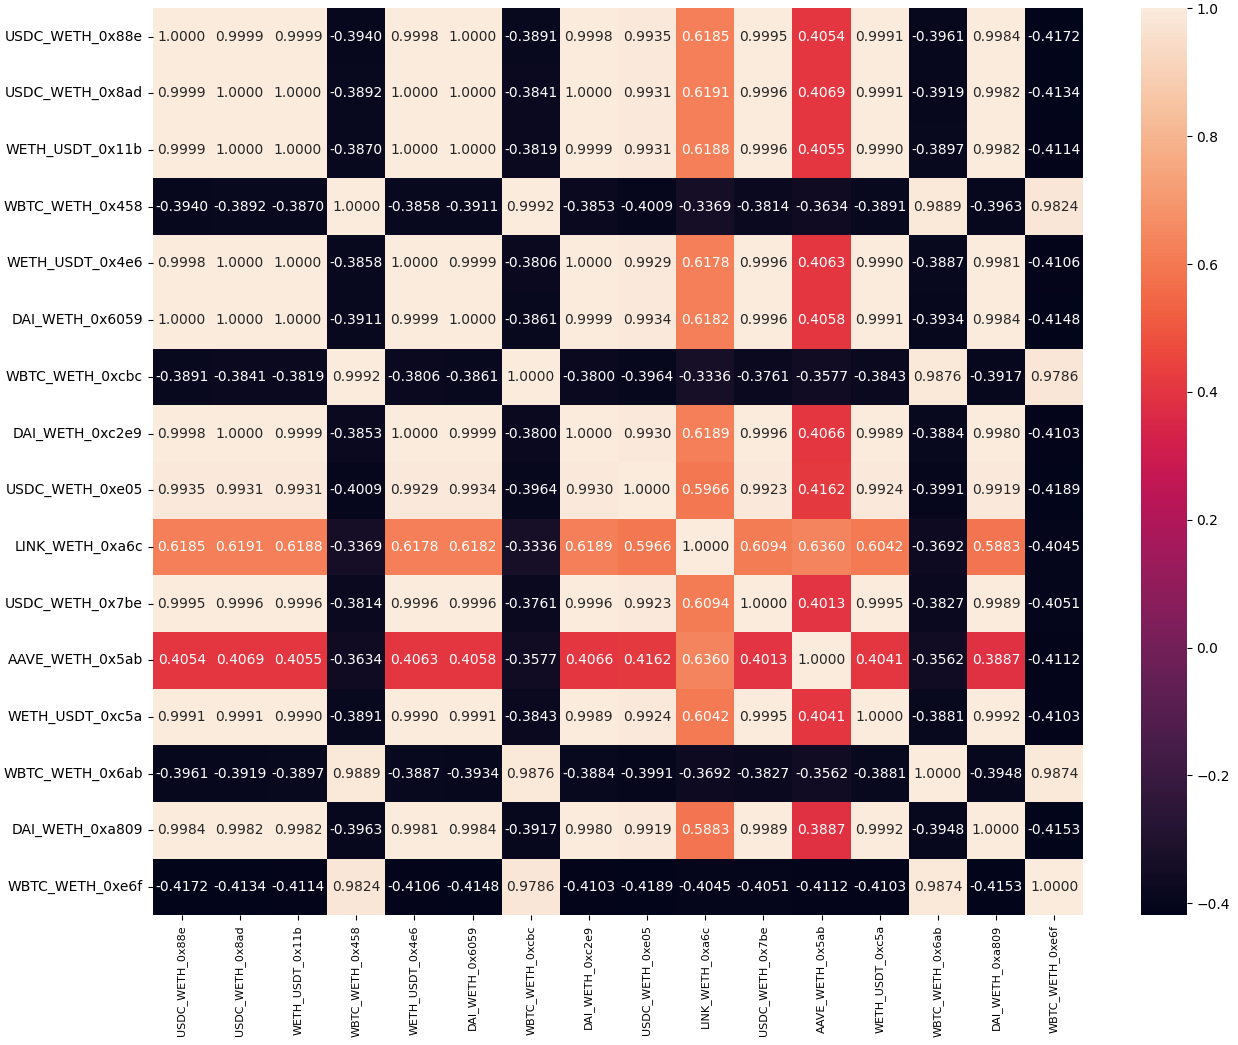
\includegraphics[width=\textwidth]{project/Images/correlationMatrix.png}
    \caption{Correlation Matrix of the Liquidity Pools that meet the \$10 million volume and include WETH \label{fig:correlationMatrix}}
\end{figure}
To determine which liquidity pools are cointegrated, the Engle-Granger approach is employed. The Engle-Granger test for cointegration involves several steps. Firstly, a unit root test is performed individually on each time series using methods like the Augmented Dickey-Fuller (ADF) test. These tests assess whether the time series is stationary or exhibits unit roots (non-stationary) individually. For cointegration to hold, both time series must be non-stationary.
\\[3mm]
Once it is established that both time series are non-stationary, the cointegration equation is estimated. Typically, a linear regression model captures the long-term relationship between the time series variables. This equation explains how the variables are linked over a long period.
\\[3mm]
Subsequently, a unit root test is conducted on the residuals obtained from the regression analysis. If the residuals are stationary, it is sufficient to conclude that the time series are cointegrated, implying that the variables move together in the long run, even if short-term deviations occur.
\\[3mm]
Following the sequence mentioned earlier in the Engle-Granger test enables us to determine which liquidity pools demonstrate cointegration, emphasising their interconnectedness and mutual relationship over time. The outcome of the cointegration tests for all possible combinations of liquidity pools is presented in Table \ref{tab:coin_pools}. This table provides a comprehensive list of the liquidity pool pairs, the results of their respective cointegration tests, and the correlation coefficient of each combination.
\begin{table}[!ht]
    \centering
    \begin{adjustwidth}{-1in}{-0.9in}
        \begin{tabular}{|p{12em}|p{12em}|p{5em}|p{4.2em}|p{4.2em}|p{4.2em}|p{3.5em}|}\hline
            pool1 & pool2 & t-statistic of unit-root test & \multicolumn{3}{|c|}{Critical Values} & Corr Coeff\\[-1ex]\cline{4-6}
            &   &   & 1\% & 5\% & 10\% & \\\hline
            \truncate{12em}{USDC\_WETH\_0x88e6a0c2ddd26feeb64f039a2c41296fcb3f5640} & \truncate{12em}{USDC\_WETH\_0xe0554a476a092703abdb3ef35c80e0d76d32939f} & -11.306176 & -3.898069 & -3.337038 & -3.045081 & 0.99347\\\hline
            \truncate{12em}{USDC\_WETH\_0x8ad599c3a0ff1de082011efddc58f1908eb6e6d8} & \truncate{12em}{USDC\_WETH\_0xe0554a476a092703abdb3ef35c80e0d76d32939f} & -11.210146 & -3.898082 & -3.337046 & -3.045086 & 0.99307\\\hline
            \truncate{12em}{WETH\_USDT\_0x11b815efb8f581194ae79006d24e0d814b7697f6} & \truncate{12em}{USDC\_WETH\_0xe0554a476a092703abdb3ef35c80e0d76d32939f} & -10.010746 & -3.898069 & -3.337038 & -3.045081 & 0.99315\\\hline
            \truncate{12em}{WETH\_USDT\_0x4e68ccd3e89f51c3074ca5072bbac773960dfa36} & \truncate{12em}{USDC\_WETH\_0xe0554a476a092703abdb3ef35c80e0d76d32939f} & -9.913205 & -3.898081 & -3.337045 & -3.045085 & 0.99291\\\hline
            \truncate{12em}{DAI\_WETH\_0x60594a405d53811d3bc4766596efd80fd545a270} & \truncate{12em}{USDC\_WETH\_0xe0554a476a092703abdb3ef35c80e0d76d32939f} & -11.395276 & -3.898069 & -3.337038 & -3.045081 & 0.99338\\\hline
            \truncate{12em}{DAI\_WETH\_0xc2e9f25be6257c210d7adf0d4cd6e3e881ba25f8} & \truncate{12em}{USDC\_WETH\_0xe0554a476a092703abdb3ef35c80e0d76d32939f} & -10.418722 & -3.89831 & -3.337173 & -3.045174 & 0.99298\\\hline
            \truncate{12em}{USDC\_WETH\_0xe0554a476a092703abdb3ef35c80e0d76d32939f} & \truncate{12em}{WETH\_USDT\_0xc5af84701f98fa483ece78af83f11b6c38aca71d} & -9.7789 & -3.901414 & -3.338902 & -3.046374 & 0.99243\\\hline
        \end{tabular}
    \end{adjustwidth}
    \caption{Cointegration test on Liquidity Pool pairs \label{tab:coin_pools}}
\end{table}
\vspace{-3mm}
\noindent By concentrating on the cointegrated pairs, we can delve deeper into exploring their dynamics, assessing their behaviour, and leveraging the interconnectedness between these liquidity pools. This approach enables us to prioritise our analysis and concentrate on the most relevant liquidity pool combinations that offer potential opportunities for profitable trading or other related activities.

